%% 1. DUAL-DISPLAY NOTES:
%\documentclass[hyperref={bookmarks=false}]{beamer}
%\usepackage{pgfpages}
%\setbeameroption{show notes on second screen=left}

% 2. NOTES ON SEPARATE SLIDES:
%\documentclass[xcolor=dvipsnames,9pt,show notes]{beamer}

% 3. NOTES ONLY:
%\documentclass[xcolor=dvipsnames,9pt,show only notes]{beamer}

% 4. HANDOUTS:
%\documentclass[xcolor=dvipsnames,9pt,handout,show notes]{beamer}

% 5. NO NOTES: ONLY ONE THAT BUILDS WITHOUT WARNINGS
\documentclass[xcolor=dvipsnames,9pt,hide notes,mathserif]{beamer}
%\setbeameroption{show only notes}
%\setbeameroption{show notes}
\usepackage{enumerate,amsmath,amssymb,fancyhdr,mathrsfs,amsthm,url,stmaryrd}
\usepackage{pgfpages}
\usepackage{listings}

%% For creating a handout:
%\pgfpagesuselayout{4 on 1}[border shrink=5mm]
%\mode<handout>{\setbeamercolor{background canvas}{bg=black!5}}

\setbeamerfont{structure}{family=\rmfamily,shape=\scshape} 
\usepackage{graphicx}
\usepackage{tikz}
\usepackage{scalefnt}
\usetikzlibrary{matrix,arrows}

\usepackage{mathrsfs,textcomp}
\setbeamertemplate{navigation symbols}{}
\usepackage{verbatim}
\usepackage[mathcal]{euscript}

\definecolor{Crimson}{rgb}{0.800,0.000,0.200}
\definecolor{darkred}{rgb}{0.5,0,0}
\newcommand{\Alert}[1]{\textcolor{darkred}{{\bf \emph{#1}}}}
\renewcommand{\alert}[1]{\textcolor{darkred}{\emph{#1}}}
\newcommand{\bs}{\ensuremath{\backslash}}
\newcommand{\Eq}{\ensuremath{\operatorname{Eq}}}
\newcommand{\Con}{\ensuremath{\operatorname{Con}}}
\newcommand{\Sub}{\ensuremath{\operatorname{Sub}}}
\newcommand{\NSub}{\ensuremath{\operatorname{NSub}}}
\renewcommand{\phi}{\ensuremath{\operatorname{\varphi}}}
\renewcommand{\leq}{\ensuremath{\leqslant}}
\renewcommand{\nleq}{\ensuremath{\nleqslant}}
\renewcommand{\geq}{\ensuremath{\geqslant}}
\renewcommand{\gneq}{\ensuremath{\gneqslant}}
\renewcommand{\ngeq}{\ensuremath{\ngeqslant}}
\newcommand{\ssubnormal}{\ensuremath{\vartriangleleft}}
\newcommand{\subnormal}{\ensuremath{\trianglelefteqslant}}
\newcommand{\supnormal}{\ensuremath{\trianglerighteqslant}}
\newcommand{\notsubnormal}{\ensuremath{\ntrianglelefteqslant}}
\newcommand{\circone}{\ensuremath{\circ^{1}}}
\newcommand{\circtwo}{\ensuremath{\circ^{2}}}
\newcommand{\circthree}{\ensuremath{\circ^{3}}}
\newcommand{\circfour}{\ensuremath{\circ^{4}}}
\newcommand{\circi}{\ensuremath{\circ^{i}}}
\newcommand{\circj}{\ensuremath{\circ^{j}}}
\newcommand{\circn}{\ensuremath{\circ^{n}}}
\newcommand{\acb}{\ensuremath{\alpha \circn \beta}}
\newcommand{\bca}{\ensuremath{\beta \circn \alpha}}

\setbeamercolor{block title example}{fg=darkred,bg=white} %orange!20!black}

\usecolortheme[named=darkred]{structure} 
\setbeamertemplate{items}[ball] 
\setbeamertemplate{blocks}[rounded][shadow=true] 

\mode<presentation>{\usetheme{boxes}}

\usepackage[english]{babel}
\usepackage[latin1]{inputenc}
\usepackage{times}
\usepackage[T1]{fontenc}
% Or whatever. Note that the encoding and the font should match. If T1
% does not look nice, try deleting the line with the fontenc.

\title[Synchronizing Automata]{Dedekind's transposition principle\\
{\small and}\\
permuting subgroups \& equivalence relations\\
{\small and (maybe, but probably not)}\\
{\small isotopic algebras with nonisomorphic congruence lattices}}
\author[William DeMeo]{William DeMeo\\
{\small \url{williamdemeo@gmail.com}}
}
\institute[\url{williamdemeo@gmail}]{{\small {\color{darkred}  University of South Carolina}}}

\date[Zassenhaus Conference -- Asheville, NC]{
Zassenhaus Conference at WCU\\
Asheville, NC\\[6pt]
May 24--26, 2013
}

\subject{Universal Algebra; Lattice Theory.}% (optional) inserted into PDF info catalog.

% TOC pops up at the beginning of each subsection:
\AtBeginSubsection[]{
  \begin{frame}<beamer>
    \frametitle{Outline}
    \tableofcontents[currentsection,currentsubsection]
  \end{frame}
}

\setbeamercovered{opaque}

%%%% INSERT MACROS %%%%
\newcommand{\bA}{\ensuremath{\mathbf{A}}}
\newcommand{\cA}{\ensuremath{\mathcal{A}}}
\newcommand{\fA}{\ensuremath{\mathfrak{A}}}
\newcommand{\sA}{\ensuremath{\mathscr{A}}}

\newcommand{\cB}{\ensuremath{\mathcal{B}}}
\newcommand{\bB}{\ensuremath{\mathbf{B}}}
\newcommand{\bBi}{\ensuremath{\mathbf{B}_i}}
\newcommand{\sB}{\ensuremath{\mathscr{B}}}
\newcommand{\fB}{\ensuremath{\mathfrak{B}}}

\newcommand{\bC}{\ensuremath{\mathbf{C}}}
\newcommand{\bF}{\ensuremath{\mathbf{F}}}
\newcommand{\sF}{\ensuremath{\mathcal{F}}}

\newcommand{\bL}{\ensuremath{\mathbf{L}}}

\newcommand{\lb}{\ensuremath{\llbracket}}
\newcommand{\rb}{\ensuremath{\rrbracket}}
\newcommand{\meet}{\ensuremath{\wedge}}
\newcommand{\join}{\ensuremath{\vee}}
\newcommand{\Meet}{\ensuremath{\bigwedge}}
\renewcommand{\Join}{\ensuremath{\bigvee}}

\newtheorem{prop}[theorem]{Proposition}
\newtheorem{assumption}[theorem]{Assumption}
\theoremstyle{definition}
\newtheorem{question}[theorem]{Question}
\newcounter{claim}
\newtheorem{claim}[claim]{Claim}
\newcounter{conjecture}
\newtheorem{conjecture}[conjecture]{Conjecture}
\newtheorem{case}{Case}
\theoremstyle{remark}
\newtheorem*{computations}{Computations}
\newtheorem*{remark}{Remark}
\newtheorem*{remarks}{Remarks}
\newtheorem*{notation}{Notation}
\numberwithin{theorem}{section}
\numberwithin{claim}{section}
\numberwithin{equation}{section}
\numberwithin{conjecture}{section}

\newcommand{\czerny}{\v{C}ern\'{y}}
\newcommand{\defn}[1]{\textcolor{darkred}{\textit{#1}}}
\newcommand{\IE}{{\small IE}}
\newcommand{\Op}{\ensuremath{\operatorname{Op}}}

\newcommand{\<}{\ensuremath{\langle}}
\renewcommand{\>}{\ensuremath{\rangle}}
\newcommand{\Clo}{\ensuremath{\mathrm{Clo}}}



%%%%%%%%%%%%  BEGIN DOCUMENT %%%%%%%%%%%%%%%

\begin{document}
\thicklines
\includeonlyframes{titlepage,A5,IntervalIsomorphisms,ExampleOfPermutingIso,intro,gsets1,gsets2,questions,equiv,answers,plug,isotopy,isotopycounters,conclusion}


%%% START HERE %%%
\frame[label=titlepage]{
  \titlepage
\vskip-3mm
  \begin{columns}
    \begin{column}{0.8\textwidth}
      \begin{center}
        {\small {\it These slides and other resources are available at}}\\[4pt]
 {\color{darkred}       \url{http://williamdemeo.wordpress.com}}
         \end{center}
       \end{column}
   \begin{column}{0.3\textwidth}
 \begin{tikzpicture}
            \node[opacity=0.9] (img2) at (2,-2){\includegraphics[height=18mm]{inputs/Dedekind-stamp}};
        \end{tikzpicture}
   \end{column}
    \end{columns}
}

\providecommand{\url}[1]{{#1}}
\providecommand{\urlprefix}{URL }


\section{Introduction}
\newcommand\dotsize{.6pt}
%% \usebackgroundtemplate{%
%% \tikz\node[opacity=0.3] {\includegraphics[height=\paperheight,widht=\paperwidth]{Dedekind-stamp}};}

%% \usebackgroundtemplate{%
%%   \vbox to \paperheight{\vfil\hbox to \paperwidth{\hfil\includegraphics[width=1.5in]{Dedekind-stamp}\hfil}\vfil}
%% }
\definecolor{olivegreen}{cmyk}{0.64,0,0.95,0.40} % PANTONE 582


\begin{frame}[fragile,label=A5]{}
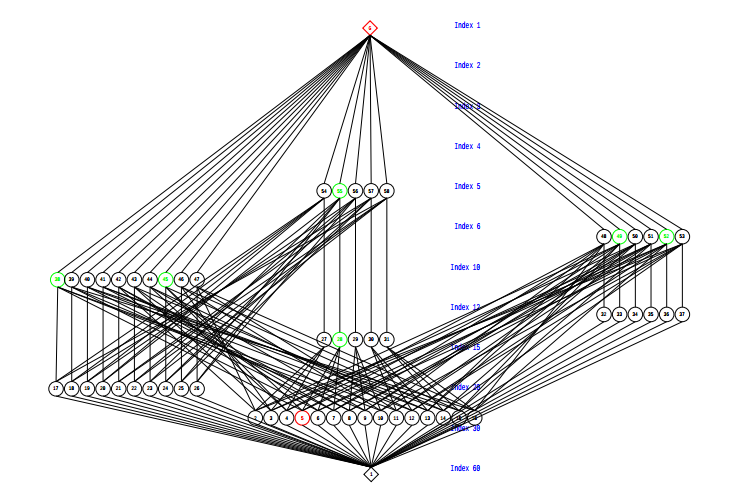
\includegraphics[width=\paperwidth]{inputs/A5}%
\end{frame}

\begin{frame}[fragile,label=IntervalIsomorphisms]{Intervals in Subgroup Lattices}
  \begin{columns}
    \begin{column}{0.3\textwidth}
%      \begin{center}

      \uncover<2->{
        {\scalefont{.9}
          \begin{tikzpicture}[scale=.4]

            \node (H) at (4,4) [draw,circle,inner sep=\dotsize] {}; \draw (H) node [right] {$K$};
            \node (U) at (-4,4) [draw,circle,inner sep=\dotsize] {}; \draw (U) node [left] {$H$};
            \node (U0) at (0,0) [draw,circle,inner sep=\dotsize] {}; 
            \draw (.7,-.5) node {$H_0 = H\cap K$};
            \node (UH) at (0,8) [draw,circle,inner sep=\dotsize] {}; \draw (UH) node
                  [above] {$\<H, K\>$};
                  \draw[semithick] (U) to [out=-10,in=100] (U0) to [out=170,in=-80] (U)
                  (UH) to [out=-10,in=100] (H) to [out=170,in=-80] (UH);
                  \draw[dotted] 
                  (H) to [out=190,in=80] (U0) to [out=10,in=-100] (H)
                  (UH) to [out=190,in=80] (U) to [out=10,in=-100] (UH);

                  \visible<2>{
                    \fill[color=darkred] 
                  %\shade[bottom color=darkred,top color=gray!-45] %            
                    (U) to [out=-10,in=100] (U0) to [out=170,in=-80] (U);
                  }

                  \visible<3,5->{
                    \shade[bottom color=darkred,top color=gray!-45] 
                  %            \fill[color=darkred]
                  (UH) to [out=-10,in=100] (H) to [out=170,in=-80] (UH);
                  }
                  \visible<4>{
                  \shade[bottom color=darkred,top color=gray!-45] %            
                    %\fill[color=darkred] 
                    (U) to [out=-10,in=100] (U0) to [out=170,in=-80] (U);
                  }

                  \visible<5->{
                  %\shade[bottom color=darkred,top color=gray!-45] %            
                   \fill[color=darkred] 
                    (U) to [out=-10,in=100] (U0) to [out=170,in=-80] (U);
                    \shade[bottom color=darkred,top color=gray!-45] 
                  %            \fill[color=darkred]
                  (UH) to [out=-10,in=100] (H) to [out=170,in=-80] (UH);
                    \node (V) at (-2.3,2.5) [fill,circle,inner sep=\dotsize] {}; \draw (V) node [left] {$X$};
                    \node (X) at (2.5,5.3) [fill,circle,inner sep=\dotsize] {}; \draw (X) node [right] {$Y$};
                  \node (VH) at (1.7,6.5)[fill,circle,inner sep=\dotsize] {}; \draw (VH) node [right] {$XK$};
                  \node (UcapX) at (-1.5,1.3)[fill,circle,inner sep=\dotsize] {};  \draw (UcapX) node [left] {$H\cap Y$};
                  \draw[semithick,->] 
                  (V) to [out=65,in=-155] (VH);
                  \draw[semithick,->] 
                  (X) to [out=-155,in=65] (UcapX);}
          \end{tikzpicture}
        }
      }

    \end{column}
    \begin{column}{0.7\textwidth}
      \begin{itemize}
      \item Let $H, K$ be subgroups of a group $G$.
      \item %Instead of $H\subnormal \<U,H\>$, assume only
        Recall the set 
        \[
        HK = \{hk \mid h\in H, \, k\in K\}
        \]
        is a group if and only if $HK = KH = \<U,H\>$.
      \item<2-> Let $H_0 = H\cap K$ and define
        \begin{equation*}
          \lb H_0, H \rb := \{ X \mid H_0 \leq X \leq  H\},
        \end{equation*}
        \uncover<3->{          
          \begin{equation*}
            \lb K, \<H,K\> \rb := \{ X \mid K \leq X \leq  \<H,K\>\}.
        \end{equation*}}
\vskip-3mm
      \item<4-> Define
        \begin{equation*}
          \lb H_0, H \rb^K := \{ X\in \lb H_0, H\rb \mid XK = KX\}.
        \end{equation*}
      \end{itemize}
    \end{column}
  \end{columns}
\vskip-3mm
  \visible<5->{
    \begin{lemma}  
\[      \text{If $HK = KH$, then 
      $\lb K, HK\rb  \cong  \lb H_0, H\rb^K \leq \lb H_0, H \rb$.}
\]
~
      %%        % \only<6>{ and \hskip2mm $[U, UH] \cong  [U_0, H]^U \leq [U_0, H]$.}\\[6pt]
      %%       \item If $U \subnormal UH$, then  $[U_0, U]_H  = [U_0, U]^H \leq [U_0, U]$.\\[6pt]
      %%       \item If $H \subnormal UH$,  then  $[U_0, U]_H  = [U_0, U]^H = [U_0, U]$.
      %%       \end{enumerate}
    \end{lemma}
  }

\note{
  \begin{itemize}
  \item 
  Since $G=UH$ is a group, the hypothesis of (ii) is equivalent to
$H\leq N_G(U)$, and the hypothesis of (iii) is equivalent to $U\leq N_G(H)$.
\item Part (i) of the lemma says that when two subgroups permute, we can
identify the interval above either one of them with the sublattice of
subgroups below the other that permute with the first.
\item Part (ii) is similar except we identify the interval above $H$ with
the  sublattice of $H$-invariant subgroups below $U$.
\item Once we have proved (i), the
proof of (iii) follows trivially from the Noether isomorphism theorem.
  \end{itemize}}

\end{frame}

%%%%%% Example2 %%%%%%%%%
\begin{frame}[fragile,label=ExampleOfPermutingIso,shrink=5]{Example}

  \begin{itemize}
  \item<1-> The group $S_4$ has permuting subgroups $H\cong D_8$ and $K\cong C_3$.
 \\{\small  (neither one normalizes the other)}
  \end{itemize}
\vskip4mm
\visible<2->{
\begin{center}
  {\scalefont{.8}
    \begin{tikzpicture}[scale=.4]
      
        \node (U0) at (0,0)  [draw, circle, inner sep=\dotsize] {};
        \draw (U0) node [below] {$H_0 = 1$};
        \node (UH) at (3,13)  [draw, circle, inner sep=\dotsize] {};
        \draw (UH) node [above] {$HK = S_4$};
        \node (V) at (-3,5)  [draw, circle, inner sep=\dotsize] {};
        \node (W) at (1,5)  [draw, circle, inner sep=\dotsize] {};
        \node (U) at (-2,8)  [draw, circle, inner sep=\dotsize] {};
        \draw (U) node [left] {$H\cong D_8$};
        \node (H) at (5,5)  [draw, circle, inner sep=\dotsize] {};
        \draw (H) node [right] {$K \cong C_3$};
        \node (A4) at (2,10)  [draw, circle, inner sep=\dotsize] {};
        \draw (A4) node [right] {$A_4$};
        \node (S3) at (6,10)  [draw, circle, inner sep=\dotsize] {};
        \draw (S3) node [right] {$S_3$};
        \node (a) at (-3.6,3)  [draw, circle, inner sep=\dotsize] {};
        \node (b) at (-2,3)  [draw, circle, inner sep=\dotsize] {};
        \node (c) at (-1,4)  [draw, circle, inner sep=\dotsize] {};
        \node (d) at (-0,4)  [draw, circle, inner sep=\dotsize] {};
        \node (e) at (-1.5,6)  [draw, circle, inner sep=\dotsize] {};
        \node (f) at (0,6)  [draw, circle, inner sep=\dotsize] {};

        \draw[semithick] 
        (U0) to (a) to (V) to (b) to (U0) to (c) to (V) to (U) to (e) to (c) to
        (f) to (d) to (U0) to (W) to (f) to (U) (UH) to (A4) to (H) to (S3)
        to (UH);
        \draw[semithick,dotted] 
        (U) to (UH)   (U0) to (H);
       %\draw (-4.5,2.2) node {$L \cong$};



      \visible<3->{\draw[semithick,dotted]
        (V) to (A4) (W) to (S3);
        \draw (V) node [left] {$C_2\times C_2$};
        \draw (W) node [right] {$C_2 $};
      }
    \end{tikzpicture}
  }
\end{center}
}
\begin{itemize}
\item<2-> Only four subgroups of $H$ permute with $K$%
\visible<3->{, including
    \[ 
H\cap A_4 \cong C_2\times C_2, \qquad H \cap S_3 \cong C_2.
    \]
  }
\end{itemize}
\end{frame}



%%% SLIDE 1 %%%
\begin{frame}[label=intro]{Dedekind's Transposition Principle}{for modular
    lattices}

  \begin{columns}
    \begin{column}{0.65\textwidth}
      {\bf Notation}

      \vskip2mm

      Let $\bL = \<L, \meet, \join\>$ be a lattice with $a \in L$.  

      \vskip2mm

      Let $\phi_a$ and $\psi_a$ be the ``perspectivity maps''
      \[
      \phi_a(x) = x\meet a \quad \text{ and }\quad 
      \psi_a(x) = x\join a
      \]
    For $x, y \in L$, let $\lb x, y \rb_L = \{ z\in L \mid x \leq z \leq
      y\}$.
    \end{column}

    \begin{column}{0.4\textwidth}
      \uncover<2->{
        {\scalefont{.9}
          \begin{tikzpicture}[scale=.4]

            \node (H) at (4,4) [draw,circle,inner sep=\dotsize] {}; \draw (H) node [right] {$b$};
            \node (U) at (-4,4) [draw,circle,inner sep=\dotsize] {}; \draw (U) node [left] {$a$};
            \node (U0) at (0,0) [draw,circle,inner sep=\dotsize] {}; 
            \draw (.7,-.5) node {$a\meet b$};
            \node (UH) at (0,8) [draw,circle,inner sep=\dotsize] {}; \draw (UH) node
                  [above] {$a\join b$};
                  \draw (U) to [out=-10,in=100] (U0) to [out=170,in=-80] (U)
                  (UH) to [out=-10,in=100] (H) to [out=170,in=-80] (UH);
                  \draw[dotted] 
                  (H) to [out=190,in=80] (U0) to [out=10,in=-100] (H)
                  (UH) to [out=190,in=80] (U) to [out=10,in=-100] (UH);

                  \shade[bottom color=darkred,top color=gray!-45] %            \fill[color=darkred] 
                  (U) to [out=-10,in=100] (U0) to [out=170,in=-80] (U);
                  \shade[bottom color=darkred,top color=gray!-45] 
                  %            \fill[color=darkred]
                  (UH) to [out=-10,in=100] (H) to [out=170,in=-80] (UH);
                  \node (V) at (-2.3,2.5) [fill,circle,inner sep=\dotsize] {}; \draw (V) node [left] {$x$};
                  \node (VH) at (1.7,6.5)[fill,circle,inner sep=\dotsize] {}; \draw (VH) node [right] {$\psi_b(x)$};
                  \node (X) at (2.5,5.3) [fill,circle,inner sep=\dotsize] {}; \draw (X) node [right] {$y$};
                  \node (UcapX) at (-1.5,1.3)[fill,circle,inner sep=\dotsize] {};  \draw (UcapX) node [left] {$\phi_a(y)$};
                  \draw[semithick,->] 
                  (V) to [out=65,in=-155] (VH);
                  \draw[semithick,->] 
                  (X) to [out=-155,in=65] (UcapX);
          \end{tikzpicture}
        }
      }
    \end{column}
  \end{columns}

  \vskip4mm


\uncover<2->{
\begin{columns}
    \begin{column}{0.75\textwidth}
%      \begin{center}
  \begin{theorem}[Dedekind's Transposition Principle]
    $\bL$ is modular iff for all $a, b\in L$ the maps $\phi_a$ and $\psi_b$ are
    inverse lattice isomorphisms of $\lb a\meet b, a \rb$ and $\lb b, a\join b\rb$.

~
  \end{theorem}
   \end{column}
 
   \begin{column}{0.25\textwidth}
 %% \begin{tikzpicture}
 %%            \node[opacity=0.5] (img2) at (2,-2){\includegraphics[height=18mm]{Dedekind-stamp}};
 %%        \end{tikzpicture}

    \end{column}
\end{columns}
}

%% \end{columns}
\end{frame}

%%% SLIDE 2 %%%
\begin{frame}[label=intro,shrink=5]{Another Transposition Principle}
{for lattices of equivalence relations}
Let $X$ be a set and let $\Eq X$ be the lattice of equivalence relations on $X$.  

\vskip2mm

Given $\alpha, \beta \in \Eq X$, define the \alert{composition} of $\alpha$ and
$\beta$ to be the binary relation
\[
\alpha \circ \beta = \{(x,y)\in X^2 \mid (\exists z\in X) \, x \mathrel{\alpha} z \mathrel{\beta} y\}.
\]
%% Note that $\circ$ is associative:
%% $(\alpha \circ \beta) \circ \gamma = \alpha \circ (\beta \circ \gamma)$.
%% \vskip2mm

%% Given $\alpha, \beta \in \Eq X$ with $\alpha\leq \beta$, define
%% the
%% \emph{interval sublattice of equivalence relations above $\alpha$ and below
%%   $\beta$}, denoted $\lb \alpha, \beta \rb$, as follows:
%% \[
%% \lb \alpha, \beta\rb:= \{\gamma \in \Eq X \mid \alpha \leq \gamma \leq \beta\}.
%% \]

%% \vskip2mm

For a sublattice $L\leq \Eq X$, with $\eta,
\theta \in L$,  define

\[
\lb \eta, \theta\rb_L = \{\gamma \in L \mid \eta \leq \gamma \leq \theta\},
\]

%% let $\lb \alpha, \beta \rb_L:= \lb \alpha, \beta \rb \cap L$,
%% denote the \emph{interval of $L$ above $\alpha$ and below $\beta$}.

\vskip-1mm

\uncover<2->{
%For $\beta \in \Eq X$, let 
%let  $\lb \alpha, \beta \rb_L^\beta$ denote
\[
\lb \eta, \theta \rb_L^\beta = \{\gamma \in L \mid \eta \leq \gamma \leq
\theta \text{ and } \gamma \circ \beta = \beta \circ \gamma\},
\]
i.e.,  the relations in $\lb \eta, \theta \rb_L$  that permute with $\beta$.
}
\vskip-4mm
\uncover<3->{
\begin{columns}
    \begin{column}{0.7\textwidth}
%      \begin{center}
\begin{lemma}
\label{lem:1}
Suppose $\alpha$ and $\beta$ are permuting relations in $L\leq \Eq X$.
% and $\alpha\circ \beta = \beta \circ\alpha$. Then
% \begin{equation}
%   \label{eq:0}
\[\text{Then } \; \lb\beta, \alpha \join \beta\rb_L \cong \lb\alpha \meet \beta, \alpha\rb_L^\beta \leq 
\lb\alpha \meet \beta, \alpha\rb_L.
\]
\end{lemma}
    \end{column}
 
   \begin{column}{0.3\textwidth}
        {\scalefont{.9}
          \begin{tikzpicture}[scale=.35]

            \node (H) at (4,4) [draw,circle,inner sep=\dotsize] {}; \draw (H) node [right] {$\beta$};
            \node (U) at (-4,4) [draw,circle,inner sep=\dotsize] {}; \draw (U) node [left] {$\alpha$};
            \node (U0) at (0,0) [draw,circle,inner sep=\dotsize] {}; 
            \draw (1,-.5) node {$\alpha \meet \beta$};
            \node (UH) at (0,8) [draw,circle,inner sep=\dotsize] {}; \draw (UH) node
                  [above] {$\alpha \join \beta$};
                  \draw (U) to [out=-10,in=100] (U0) to [out=170,in=-80] (U)
                  (UH) to [out=-10,in=100] (H) to [out=170,in=-80] (UH);
                  \draw[dotted] 
                  (H) to [out=190,in=80] (U0) to [out=10,in=-100] (H)
                  (UH) to [out=190,in=80] (U) to [out=10,in=-100] (UH);

                  %\shade[bottom color=darkred,top color=gray!-45] %            
                  \fill[color=darkred] 
                  (U) to [out=-10,in=100] (U0) to [out=170,in=-80] (U);
                  \shade[bottom color=darkred,top color=gray!-45] 
                  %            \fill[color=darkred]
                  (UH) to [out=-10,in=100] (H) to [out=170,in=-80] (UH);
                  \node (V) at (-2.5,2.7) [fill,circle,inner sep=\dotsize] {}; \draw (V) node [left] {$x$};
                  \node (VH) at (2,6.75)[fill,circle,inner sep=\dotsize] {};
                  \draw (3,7.2) node {$x \circ \beta$};
                  \node (X) at (2.5,5.3) [fill,circle,inner sep=\dotsize] {}; \draw (X) node [right] {$y$};
                  \node (UcapX) at (-1.78,1.2)[fill,circle,inner sep=\dotsize] {};  %\draw (UcapX) node [left] {$\alpha\meet y$};
                  \draw (-2.6,.4) node {$y \meet \alpha$};
                  \draw[semithick,->] 
                  (V) to [out=65,in=-155] (VH);
                  \draw[semithick,->] 
                  (X) to [out=-155,in=65] (UcapX);
          \end{tikzpicture}
      }

    \end{column}
\end{columns}
}
\uncover<4>{\alert{Question:} Does this generalize the subgroup lattice lemma?}
\end{frame}

%%% SLIDE 5 %%%
\begin{frame}[label=gsets1]{Answer}
\begin{center}
\uncover<1->{Yes!}
\vskip1cm
\uncover<2->{<insert G-set stuff here>}
\end{center}
\uncover<3->{
\begin{lemma}
  In $\Con \<G\bs H, \bar{G}\>$, two congruences $\theta_{K_1}$ and $\theta_{K_2}$
  permute if and only if the corresponding subgroups $K_1$ and $K_2$ permute.
\end{lemma}}
\end{frame}




%%% SLIDE 6 %%%
\begin{frame}[label=questions]{Questions}
Recall that $HK = \<H,K\>$ if and only if $HK = KH$.
\vskip3mm
\uncover<2->{
{\bf Question 1.} Is it true that
\begin{quote}
$HKH = \<H,K\>$ if and only if $HKH = KHK$?
\end{quote}}
\uncover<3->{What about
\begin{quote}
$HKHK = \<H,K\>$ if and only if $HKHK = KHKH$?
\end{quote}}
\uncover<4->{
  \begin{center}
  $\vdots$
  \end{center}
\begin{quote}
%$HKH\cdots K = \<H,K\>$ 
$H\circn K = \<H,K\>$ if and only if $H \circn K = K\circn H$? %$HKH\cdots K = KHK\cdots H$?
\end{quote}}
\end{frame}





%%% SLIDE 7 %%%
\begin{frame}[label=questions]{Questions}
Denote  by $H\circn K$ the \emph{$n$-fold composition of $H$ and $K$}.%\vskip-2mm
\begin{align*}
%% \text{Define} \qquad 
H \circone K &= H,\\
H \circtwo K &= HK,\\
H \circthree K &= HKH,\\
H \circfour K &= HKHK,\\
&\vdots\\
H \circn K &= H\circtwo K \circ^{n-1}H.
\end{align*}
We say $H$ and $K$ are \alert{$n$-permuting} if $H\circn K = K\circn H$.\\[4pt]
\uncover<2->{
{\bf Question 2.} {\it Is the following true?}
\begin{quote}
If $H$ and $K$ are $n$-permuting, then interval $\lb K, \<H,K\>\rb$ 
is isomorphic to the lattice of subgroups in $\lb H_0, H\rb$ that $n$-permute
with $K$.
\end{quote}
}
\end{frame}


%%% SLIDE 8 %%%
\begin{frame}[label=equiv]{Connection with equivalence relations}
Let $\bA = \<H \backslash G, \bar{G}\>$ be the algebra with
\begin{itemize}
\item  universe: the right cosets $H\bs G = \{Hx \mid x\in G\}$ \\[4pt]
\item operations: $\bar{G} = \{g^{\bA} : g\in G\}$, where $g^{\bA}(Hx)=Hxg$.
\end{itemize}

\uncover<2->{
  \begin{lemma}
The subgroups $K_1$ and $K_2$ are $n$-permuting if and only if their corresponding
congruences $\theta_{K_1}$ and $\theta_{K_2}$ are $n$-permuting.
That is,
\[
K_1\circn K_2 = K_2 \circn K_1
\iff
\theta_{K_1} \circn \theta_{K_2}  = \theta_{K_2} \circn \theta_{K_1}.
\]
%    Let $\theta_H$ and $\theta_K$ be equivalence relations on a set $X$.
  \end{lemma}}
\end{frame}


%%% SLIDE 8 %%%
\begin{frame}[label=answers,shrink=5]{Answer to Question 1.}
\begin{lemma}
For $\alpha, \beta \in \Eq X$, and for every \alert{even} integer $n>1$, TFAE:
 %% \begin{enumerate}[(i)]
 %% \item $\theta_H \circn \theta_K = \theta_H \join \theta_K$
 %% \item $\theta_H \circn \theta_K = \theta_K \circn \theta_H$
 %% \item $\theta_H \circn \theta_K \subseteq \theta_K \circn \theta_H$
 %% \end{enumerate}
 \begin{enumerate}[(i)]
 \item $\alpha \circn \beta = \alpha \join \beta$
 \item $\alpha \circn \beta = \beta \circn \alpha$
 \item $\alpha \circn \beta \subseteq \beta \circn \alpha$
 \end{enumerate}
% \[ \alpha\circn \beta = \alpha \join \beta \iff \alpha\circn \beta = \beta \circn \alpha. \]
\end{lemma}
\uncover<2->{
For $n=3$,
\[
%% \alpha \circthree \beta = \beta \circthree \alpha\; \Longrightarrow \;
%% \alpha \circthree \beta = \alpha \join \beta\]
\alpha \circ \beta \circ \alpha = \beta \circ \alpha \circ \beta\quad \Longrightarrow \quad
\alpha \circ \beta\circ \alpha = \alpha \join \beta\]
but the converse is false.
}
\uncover<3->{
\begin{corollary}
For $H, K \leq G$, and for every \alert{even} integer $n>1$, TFAE:
 \begin{enumerate}[(i)]
 \item $H \circn K = \<H, K\>$
 \item $H \circn K = K \circn H$
 \item $H \circn K \subseteq K \circn H$
 \end{enumerate}
% \[ \alpha\circn \beta = \alpha \join \beta \iff \alpha\circn \beta = \beta \circn \alpha. \]
\end{corollary}
}
\uncover<4->{
For $n=3$,
\[
HKH = KHK\quad \Longrightarrow \quad
HKH = \<H, K\>\]
but the converse is false. \\
}
\uncover<5->{{\bf Question 1.'} What are conditions on $G$ under which the converse is true?}
\end{frame}


%%% SLIDE 8 %%%
\begin{frame}[label=answers]{Answer to Question 1.}{case $n=5$}

{\bf Question 1.} Is it true that
\begin{quote}
$H\circ^5 K = \<H,K\>$ if and only if $H\circ^5 K = K\circ^5 H$?
\end{quote}
\vskip2mm
\uncover<2->{    
{\bf Answer. } No.
\vskip1cm
}
\uncover<2->{{\bf Example.}
Let $G = (C_3 \times C_3) : C_4$.\\[4pt]
This is a group of order 36 with generators $f_1, f_2, f_3, f_4$.\\[4pt]
Let $H = \<f_1\> \cong C_2$, and $K = \<f_1\cdot f_3\cdot f_4^2, f_2\cdot
f_4^2\>\cong C_4$.  Then,
\begin{itemize}
\item $H \cap K = 1$
\item $\<H, K\> = K \circ^5 H$ has order 36 so it is the whole group.
\item The \emph{set} $H \circ^5 K$ has size 34, so does not generate $\<H,K\>$.
\item $H$ covers 1.
\end{itemize}
}

\end{frame}



%%% SLIDE 8 %%%
\begin{frame}[label=answers]{Answer to Question 2.}

%% {\bf Question 2.} {\it Is the following true?}
%% \begin{quote}
%% If $H$ and $K$ are $n$-permuting, then interval $\lb K, \<H,K\>\rb$ 
%% is isomorphic to the lattice of subgroups in $\lb H_0, H\rb$ that $n$-permute
%% with $K$.
%% \end{quote}
%% }\uncover<2->{
{\bf No.}  
\begin{quote}
In general, it is not true that if $H$ and $K$ are $n$-permuting,
then the interval $\lb K, \<H,K\>\rb$ is isomorphic to the lattice of those subgroups
in $\lb H_0, H\rb$ that $n$-permute with $K$.
\end{quote}

\vskip1cm

\uncover<2->{{\bf Example.}
The group $A_5$ has subgroups
$H \cong D_{10}$, and $K \cong C_2$ such that 
\[
H\circfour K = K \circfour H = A_5,\]
but the map
\[
\lb K, A_5\rb \ni J \mapsto J\cap H \in \lb 1, H\rb
\]
is not one-to-one.
}


\end{frame}


\begin{frame}[fragile,label=A5]{Examples}
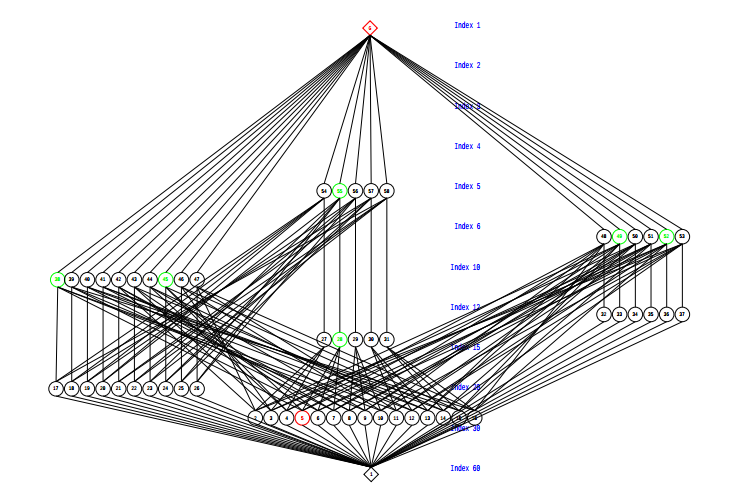
\includegraphics[width=\paperwidth]{inputs/A5}%
\end{frame}

\begin{frame}[label=answers]{Revised Question 2.}

{\bf Question 2.'} 
\begin{quote}
What are conditions on the group $G$ so that
\vskip3mm
if $H, K$ are $n$-permuting subgroups of $G$, then
\[
\lb K, \<H,K\>\rb \cong \lb H_0, H\rb^{ K \circn} \leq \lb H_0, H\rb \, ?
\]
\end{quote}
\end{frame}

\begin{frame}[fragile,label=plug]{{\tiny  <advertisement> }}
  \begin{center}
\alert{Workshop on Computational Universal Algebra}
\vskip3mm
Friday, October 4, 2013
\vskip3mm
University of Louisville, KY
\vskip3mm
\large{{\tt universalalgebra.wordpress.com}}
%% \vskip4mm
%% \includegraphics[width=12cm]{WorkshopPlug}%
  \end{center}
\end{frame}









%\begin{remarks}
%%% SLIDE 2 %%%
\begin{frame}[label=dedekind]{Dedekind's Rule}
%\begin{remarks}
\note{
  The lemma states that the sublattice $\lb\beta, \alpha \join \beta\rb_L$ is isomorphic to the 
lattice, $\lb\alpha \meet \beta, \alpha\rb_L^\beta$, of relations in $L$ that are below
$\alpha$, above $\alpha \meet \beta$, and permute with $\beta$; moreover, $\lb\alpha \meet \beta,
\alpha\rb_L^\beta$ is a sublattice of
$\lb\alpha \meet \beta, \alpha\rb_L$.
}
The proof requires the following version of \emph{Dedekind's Rule:}
\note{In the group theory setting, the well known Dedekind's
  Rule states that if $A, B, C$ are subgroups of a group,
  and $A\leq B$, then we have the following identity of sets: $A(B\cap C) = B
  \cap AC$.}
\begin{lemma}
\label{lem:dedekind}
Suppose $\alpha, \beta, \gamma \in L \leq \Eq X$ and $\alpha
\leq \beta$.
\vskip2mm
Then the following identities of subsets of $X^2$ hold:
\begin{equation*}
  \label{eq:1}
  \alpha \circ (\beta \cap \gamma) = \beta \cap (\alpha \circ \gamma)
\end{equation*}
\begin{equation*}
  \label{eq:2}
  (\beta \cap \gamma) \circ \alpha = \beta \cap (\gamma \circ \alpha)
\end{equation*}
\end{lemma}
%% \begin{proof}
%% We prove~(\ref{eq:1}); the proof of (\ref{eq:2}) is similar.  

\end{frame}

%%% SLIDE 4 %%%
\begin{frame}[label=isotopy]{Isotopy}{basic definitions}
Let $\bA$, $\bB$, $\bC$ be algebras of the same type.


\vskip2mm

$\bA$ and $\bB$ are \alert{isotopic over} $\bC$, denoted $\bA\sim_{\bC}\bB$,
if there is an isomorphism 
\[
\phi: \bA \times \bC \stackrel{\cong}{\longrightarrow} \bB \times \bC \quad
\text{ that leaves the second coordinate fixed }
\]
\[
% \text{ i.e. } \; (\forall a\in A)\,(\forall c\in C) \; \phi(a,c) = (b,c)
% \text{ for some $b \in B$.}
\text{ i.e. } \; \phi(a,c) = (b,c)\;
\text{ for some $b \in B$.}
\]

\vskip2mm
\uncover<2->{
  We say that $\bA$ and $\bB$ are \alert{isotopic}, denoted $\bA\sim \bB$, if
  $\bA\sim_{\bC}\bB$ for some $\bC$.  
  \vskip2mm
}
\alt<2>{It is easy to verify that $\sim$ is an equivalence relation.
}{
  \onslide<3->{
    If $\bA\sim_{\bC}\bB$ and $\Con (\bA \times \bC)$ happens to
    be modular, then we write}
}
\uncover<3->{
$\bA \sim^{\mathrm{mod}}_{\bC} \bB$ and say that
$\bA$ and $\bB$ are \alert{modular isotopic over} $\bC$.
\vskip2mm
}
%\onslide<4->{
\note{We call $\bA$ and $\bB$ \alert{modular isotopic in one step},  denoted 
$\bA \sim^{\mathrm{mod}}_1 \bB$,
if they are modular isotopic over some $\bC$.
\vskip2mm
}
\note{ %\onslide<5->{
We call $\bA$ and $\bB$ are \alert{modular isotopic}, denoted 
$\bA \sim^{\mathrm{mod}} \bB$, if $(\bA, \bB)$ is in the transitive
closure of $\sim^{\mathrm{mod}}_1$.
}

\end{frame}

%%% SLIDE 5 %%%
\begin{frame}[label=isotopy]{Isotopy}{modular case}
%A well known 
%\vskip2mm
%~ \hskip 2cm 
{\bf Lemma.}\hskip2mm If $\bA \sim^{\mathrm{mod}}_{\bC} \bB$ then $\Con \bA \cong \Con \bB$.

\vskip2mm

The proof is a nice/easy application of Dedekind's Transposition Principle.  

\vskip2mm
\uncover<2->{
Could we use the same strategy with the non-modular version of the transposition principle to show that 
$\bA\sim\bB$ implies $\Con \bA \cong \Con \bB$?
}
\vskip2mm

\uncover<3->{No!

\vskip2mm
The perspectivity map, which is so useful
  when $\Con (\bA\times \bC)$ is modular, can fail \emph{miserably} in the non-modular
  case...
\uncover<4->{ 
\emph{even when} $\bA \cong \bB$! } }

\vskip2mm
\uncover<5->{But this only shows that the same argument doesn't work...}

\end{frame}

%%% SLIDE 6 %%%
\begin{frame}[label=isotopycounters]{Examples}{in which $\bA\sim \bB$ and $\Con \bA \ncong \Con \bB$} 

  \vskip2mm
\note{  The examples show that congruence lattices of
  isotopic algebras can differ arbitrarily in size.}

  \vskip2mm
  \uncover<2->{
    For any group $G$, let $\Sub(G)$ denote the lattice of subgroups of $G$.
%, and    let $\NSub(G)$ denote the lattice of normal subgroups of $G$.
  }
  \vskip2mm
  \uncover<3->{
    Let $S$ be any group and let $D$ denote the \emph{diagonal subgroup} of 
    $S\times S$,
\[D = \{(x,x) \mid x\in S\}\]
  }

  \uncover<4->{
    The interval $\lb D, S\times S\rb \leq \Sub(S\times S)$ 
%% which we denote by
%%       $\lb D, S\times S\rb$, %is the sublattice of $\Sub(S\times S)$ 
%%       consists of the subgroups of $S\times S$ that contain $D$.  In symbols,
%%       $\lb D, S\times S\rb = \{K \mid D \leq K \leq S\times S\}$.  
%%       This is a sublattice of $\Sub(S\times S)$ and 
      is described by the following
    }
    \vskip2mm
    \uncover<4->{
      \begin{lemma}
        \label{lem:1}
        The filter above the diagonal subgroup of $S\times S$ %in the subgroup lattice of $S\times S$
        is isomorphic to the lattice of normal subgroups of $S$. 

~
        %In symbols, $\lb D, S\times S\rb \cong \NSub(S)$.
    \end{lemma}
    }


\end{frame}

%%% SLIDE 7 %%%
%\begin{frame}[label=intro]{The example}
\begin{frame}[label=isotopycounters]{Examples}{in which $\bA\sim \bB$ and $\Con \bA \ncong \Con \bB$} 
%% Let $S$ be any finite non-Dedekind group {\small (so there exists non-normal $\<1\> < H < S$)}
%% % has a non-trivialnon-normal subgroup).

%% \vskip2mm

Let $S$ be a group, and 
%any finite non-Dedekind group {\small (so there exists non-normal $\<1\> < H < S$)}
let $G = S_1 \times S_2$, where
$S_1 \cong S_2 \cong S$. 

\vskip2mm
Let $D = \{(x_1,x_2)\in G \mid x_1 = x_2\}, \quad T_1 = S_1 \times \<1\>, \quad T_2 = \<1\>\times S_2$.
%,  thediagonal subgroup of $G$. 
\vskip1cm

% \uncover<2->{
\note{Then $D \cong T_1 \cong T_2$, and these are pair-wise complements:
\[
\<T_1, T_2\> = \<T_1,D\> = \<D, T_2\> = G
\]
\[
T_1\cap D = D\cap T_2 = T_1 \cap T_2 =
\<(1,1)\>
\]
}

\uncover<2->{
Let $\bA = \< G/T_1, G^{\bA}\> =$ the algebra with universe the left
cosets of $T_1$ in $G$, and basic operations the left multiplications by elements
of $G$. 
\vskip2mm
%\uncover<3->{
For each $g\in G$ the operation $g^{\bA} \in G^{\bA}$ is defined by
\[
g^{\bA}(xT_1) = 
(gx)T_1 \qquad ( xT_1 \in G/T_1 ).
\]
%$g^{\bA}(xT_1) = (gx)T_1$.
Define the algebra $\bC = \< G/T_2, G^{\bC}\>$ similarly.  
}
\end{frame}


%%% SLIDE 7 %%%
%\begin{frame}[label=intro]{The example}
\begin{frame}[label=isotopycounters]{Examples}{in which $\bA\sim \bB$ and $\Con \bA \ncong \Con \bB$} 
The algebra $\bB$ will have universe $B = G/D$, but we
define the action of $G$ on $B$ with a twist.
\vskip2mm
\uncover<2->{
For each $g = (g_1, g_2) \in G$,
for each $(x_1, x_2)D \in G/D$, define
\[
g^{\bB}((x_1,x_2)D) =  (g_2x_1, g_1 x_2)D.
\]
Let $\bB = \< G/D, G^{\bB}\>$, where $G^{\bB} =  \{g^{\bB} \mid g\in G\}$.
}
\vskip2mm
\uncover<3->{
Consider the binary relation 
$\phi \subseteq (A \times C) \times (B \times C)$ that associates
to each ordered pair 
\[((x_1,x_2)T_1, (y_1,y_2)T_2) \in A \times C\]
 the pair 
\[((x_2, y_1)D, (y_1,y_2)T_2) \in B \times C\]
}

\uncover<4->{
It is easy to verify that this relation is a function, and in fact 
\[
\phi \colon \bA \times \bC \rightarrow \bB \times \bC \; \text{ is an
  isomorphism.}
\]}
\uncover<5->{
\hskip-2mm Since $\phi$ leaves second coordinates fixed, %of $\phi$-related pairs are the same,
$\bA\sim_{\bC}\bB$.  
}
\end{frame}

%%% SLIDE 7 %%%
\begin{frame}[label=conclusion]{Conclusion}
Compare $\Con \bA$ and $\Con \bB$.
\vskip2mm
\uncover<2->{
$\Con \bA \cong \lb T_1, G\rb \leq \Sub(G)$, so $\Con \bA \cong \Sub(S)$.
%(see Lemma 4.20 of ALVi).
}
\vskip2mm
\uncover<3->{
$\Con \bB$ is isomorphic to the lattice of normal subgroups
of $S$.
}
\uncover<4->{
\[
\Con \bB \cong\NSub(S) \leq \Sub(S) \cong  \Con \bA
\] 
So, if $S$ is any \alert{non-Dedekind} group, $\Con \bB \ncong \Con \bA$.
\note{
    A group $G$ is called a \alert{Dedekind group} if every subgroup of $G$ is
    normal. % ---i.e., $\Sub(G) = \NSub(G)$--- 
    A \emph{non-Dedekind group} is one with a non-trivial non-normal subgroup.

    Of course this requires $G$ be nonabelian, but that is not
    sufficient.  For example, the eight element quaternion group 
    is a Dedekind group.}

  \vskip2mm

}
\vskip2mm
\uncover<5->{If $S$ is a nonabelian simple group, then $\Con \bB \cong
  \mathbf{2}$, while
$\Con \bA \cong \Sub(S)$ can be arbitrarily large.}

\end{frame}


%%% SLIDE 5 %%%
\begin{frame}[label=gsets2]{Answer}
  \begin{itemize}
  \item For groups $H \leq G$, the algebra
$\bA = \<G\backslash H, \bar{G}\>$ has
\begin{itemize}
\item  universe: the right cosets $H\bs G = \{Hx \mid x\in G\}$ \\[4pt]
\item operations: $\bar{G} = \{g^{\bA} : g\in G\}$, where $g^{\bA}(Hx)=Hxg$.
\end{itemize}
%% In other words, each $g \in G$ acts on the set of right cosets of $H$ by right
%% multiplication.
\item<2->
A standard result is % that $\Con \bA$ is isomorphic to the interval above $H$ in
%the subgroup lattice of $G$:
$\Con \bA \cong \lb H, G\rb$. % :=\{K \mid H \leq K \leq G\}.
%\]
\\[4pt]
The isomorphism $\lb H, G\rb \ni K \mapsto \theta_K \in \Con \bA$ is
  given by
\[
\theta_K = \{(Hx, Hy) \mid xy^{-1} \in K \}.
\]
The inverse isomorphism $\Con \bA \ni \theta \mapsto K_\theta \in \lb H, G\rb$ is
\[
K_\theta = \{ g\in G \mid (H, Hg) \in \theta \}.
\]
\item<3-> So every lattice property of congruence lattices
is also a lattice property of (intervals of) subgroup lattices.  
Moreover, it's easy to prove:
\begin{lemma}
  In $\Con \<G\bs H, \bar{G}\>$, two congruences $\theta_{K_1}$ and $\theta_{K_2}$
  permute if and only if the corresponding subgroups $K_1$ and $K_2$ permute.
\end{lemma}
  \end{itemize}
\end{frame}



\end{document}
